%----------------------------------------------------------------------------------------
%	SLIDE 12.
%----------------------------------------------------------------------------------------
\begin{frame}
\frametitle{Párhuzamosítás fizikában}
\framesubtitle{Általánosságban}

\begin{columns}
	\column{0.38\linewidth}
	{\small
	\begin{itemize}
		\item Szimulációs szoftverek futtatása (pl. Szám. szim., MSc -- OpenFoam, GADGET4, HOOMD-blue)
		\item Szervereken történő munka (pl. ELTE-n az onco2, tesla, atys, veo1 (ismertebb nevén `kooplex`), stb.)
		\item Szerver-klasztereken történő futtatás (pl. ELTE \textit{Atlasz} klaszter)
	\end{itemize}}
	
	\column{0.6\linewidth}
	\begin{figure}
		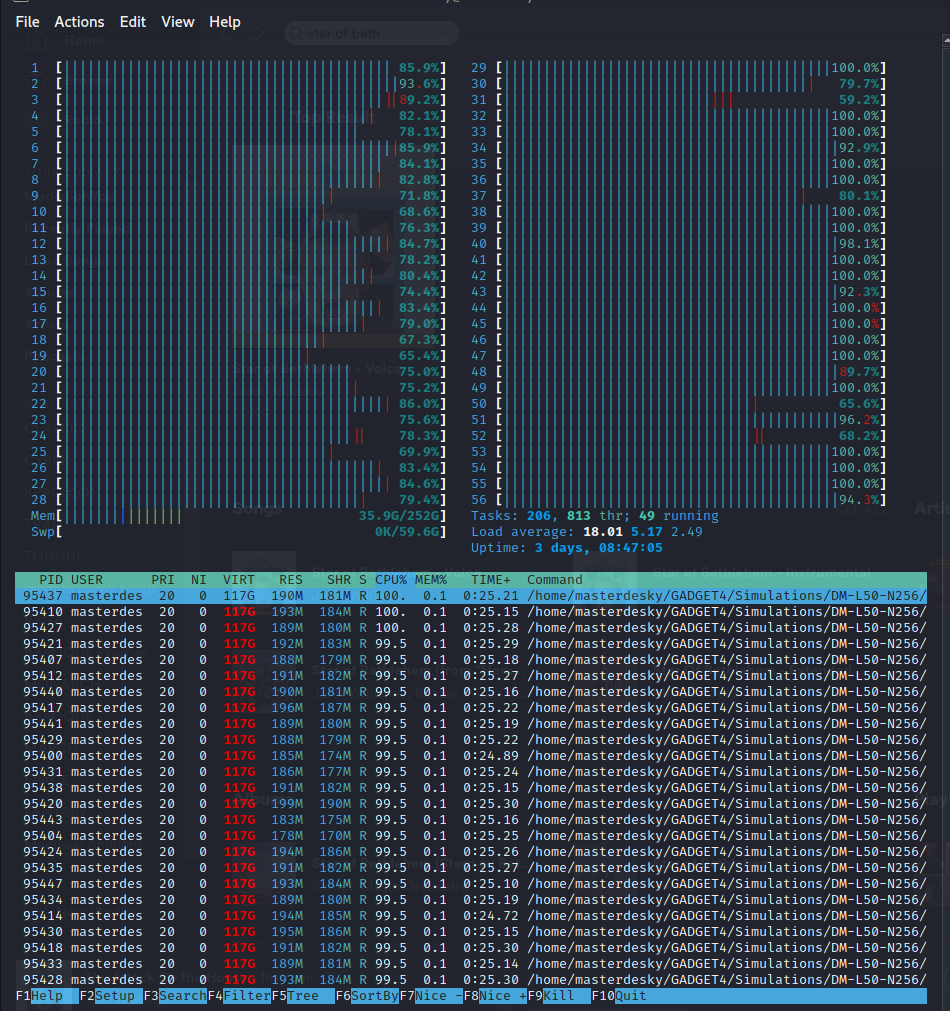
\includegraphics[width=\textwidth]{img/onco2.png}
	\end{figure}

\end{columns}

\end{frame}